\documentclass{sig-alt-hotnets}

%\usepackage{subfig}
\usepackage{subfigure}

\usepackage{multirow}

 \newcommand{\subparagraph}{} 
\usepackage[usenames,dvipsnames]{color}

\usepackage[compact]{titlesec}

\usepackage{amsmath}
\usepackage{amsfonts}


\usepackage{times}

\usepackage{xspace}
\usepackage{epsfig} 
\usepackage{amsmath}
\usepackage[hyphens]{url}
\usepackage{amsfonts} 

\usepackage{listings}
\usepackage{fancyvrb}
\VerbatimFootnotes

\setlength{\pdfpagewidth}{8.5in}
\setlength{\pdfpageheight}{11in}

\newcommand{\tightcaption}[1]{\vspace{-0.1cm}\caption{\em #1}\vspace{-0.1cm}}
\newcommand{\tightsection}[1]{\vspace{-0.15in}\section{#1}\vspace{-0.2cm}}
\newcommand{\tightsubsection}[1]{\vspace{-0.15in}\subsection{#1}\vspace{-0.2cm}}
\newcommand{\tightsubsubsection}[1]{\vspace{-0.15in}\subsubsection{#1}\vspace{-0.2cm}}

\newcommand{\eg}{{\it e.g.,}\xspace}
\newcommand{\ie}{{\it i.e.,}\xspace}

\newcommand{\comment}[1]{}
\newcounter{note}[section]
\renewcommand{\thenote}{\thesection.\arabic{note}}

\newcommand{\Section}{\S}

\usepackage{pifont}
\newcommand{\cmark}{\ding{51}}%
\newcommand{\xmark}{\ding{55}}%

\newcommand{\fillme}{{\bf XXX}~}



\newcommand{\mypara}[1]{\medskip\noindent{\bf {#1}:}~}
\newcommand{\myparatight}[1]{\smallskip\noindent{\bf {#1}:}~}
\newcommand{\myparaq}[1]{\smallskip\noindent{\bf {#1}?}~}

\newcommand{\myparaittight}[1]{\smallskip\noindent{\emph {#1}:}~}
\newcommand{\question}[1]{\smallskip\noindent{\emph{Q:~#1}}\smallskip}
\newcommand{\myparaqtight}[1]{\smallskip\noindent{\bf {#1}}~}

\newcommand{\vyas}[1]{{\footnotesize\color{red}[VS: #1]}}
\newcommand{\jc}[1]{{\footnotesize\color{red}[JC: #1]}}
%\newcommand{\seyed}[1]{{\footnotesize\color{blue}[SF: #1]}}
%\newcommand{\alig}[1]{{\footnotesize\color{BrickRed}[AG: #1]}}
%\renewcommand{\vyas}[1]{}
%\renewcommand{\seyed}[1]{}
%\renewcommand{\alig}[1]{}

\newcounter{packednmbr}

\newenvironment{packedenumerate}{\begin{list}{\thepackednmbr.}{\usecounter{packednmbr}\setlength{\itemsep}{0.5pt}\addtolength{\labelwidth}{-4pt}\setlength{\leftmargin}{\labelwidth}\setlength{\listparindent}{\parindent}\setlength{\parsep}{1pt}\setlength{\topsep}{0pt}}}{\end{list}}

\newenvironment{packeditemize}{\begin{list}{$\bullet$}{\setlength{\itemsep}{0.5pt}\addtolength{\labelwidth}{-4pt}\setlength{\leftmargin}{\labelwidth}\setlength{\listparindent}{\parindent}\setlength{\parsep}{1pt}\setlength{\topsep}{0pt}}}{\end{list}}

\newenvironment{packedtrivlist}{\begin{list}{\setlength{\itemsep}{0.2pt}\addtolength{\labelwidth}{-4pt}\setlength{\leftmargin}{\labelwidth}\setlength{\listparindent}{\parindent}\setlength{\parsep}{1pt}\setlength{\topsep}{0pt}}}{\end{list}}
%%%%%%%%%%%%
% Document %
%%%%%%%%%%%%
\begin{document}

\title{Building a Near Real-time Traffic Map for the Internet (For Free)}
%Realtime Internet Traffic Map Using Video as a Carrier}
\author{}
\maketitle

%\begin{abstract}

With the Internet traffic volume increasing rapidly and its performance more dynamic and unpredictable, real time network states have become critical for many of today's distributed systems and applications. The goal of real time measurement for Internet, though simple to state, has been tantalizingly out of reach despite of many previous attempt (iPlane/knowldge plane). It is challenging for existing methods to achieve all three of high coverage, measurement overhead and simulteneous view. In this paper, we observe a never-before-seen opportunity to address all these requirement. The key enabler is Internet video as it dominates the Internet and has become the ``background'' traffic on every major links. By measuring from video players, we will be able to collect simulteneous view of the Internet with an unprecedent high coverage. This paper outlines the vision of real-time measurement with video as a carrier and early feasible solutions to address the challenges arised from this approach.

\end{abstract}
\section{Introduction}

Many Internet services can benefit from a service that provides a real-time
global view of the state of the network---a {\em traffic map} that can predict
the available bandwidth between a pair of IP
addresses~\cite{clark2003knowledge,madhyastha2006iplane}. For instance, CDNs could implement
better server selection strategies if they could predict Internet path
properties.  Similarly, peer-to-peer applications can be more intelligent in
their choice of peers if they can predict if a specific alternative peer can
offer better performance.  Finally, websites can be optimized to choose
``mirror'' sites  or customize content for their clients if they knew the
network state.  In the absence of such a service, each application  service
provider has  to resort to expensive home-grown solutions or  operate ``in the
dark'' and hope for reasonable performance from the network or simply use
trial-and-error solutions.

 There have been many prior projects that have attempted to tackle some aspects
of this problem; e.g., predicting end-to-end paths~\cite{madhyastha2006iplane} or understanding routing reachability~\cite{katz2008studying} or designing solutions that use
fine-grained measurements to provide deeper insights into the bandwidths and
capacities of individual paths~\cite{pathneck}.  The main challenge that these
past efforts have faced can be captured along three key dimensions: 

\begin{itemize}

\item  {\em Coverage:} Obtaining a global view of the network necessarily entails deploying many millions of 
 vantage points that can run suitable measurement logic to obtain relevant path-level metrics of interest. 
 While recent work  on ``crowdsourcing'' such measurements is indeed promising~\cite{choffnes2010crowdsourcing,sanchez2013dasu,otto2011blind}, even the largest 
 deployed crowdsourced measurement efforts suffer from limited visibility.

\item {\em Overhead:}  While metrics such as reachability or latency are easy to measure,
 the more interesting metrics such as available bandwidth or capacity or the location 
 of bottleneck links have typically required carefully tuned algorithms that  incur 
 non-trivial overhead (e.g., few hundreds of kilobytes per iteration)~\cite{strauss2003measurement}.

\item {\em Real-time views:} This global 
traffic map needs to be updated in near real-time to reflect current network conditions. 
 This raises further concerns in conjunction with the coverage and overhead concerns---we need 
 millions of vantage points continuously running non-trivial measurements {\em all the time.}

\end{itemize} 


\begin{figure*}[t!]
\centering
\subfigure[Client IP prefix (/24)]
{
	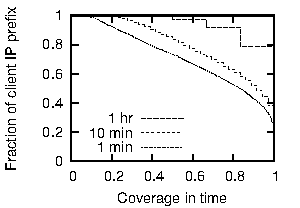
\includegraphics[width=150pt]{data2/cdf-test.pdf}
}
\hspace{-0.5cm}
\subfigure[AS]
{
	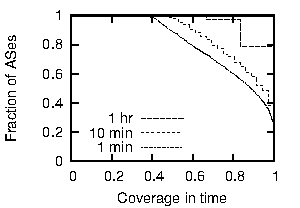
\includegraphics[width=150pt]{data2/cdf-test-clientip.pdf}
}
\hspace{-0.5cm}
\subfigure[ISP]
{
	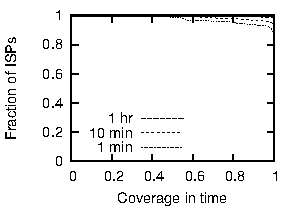
\includegraphics[width=150pt]{data2/cdf-test-isp.pdf}
}
\vspace{-0.2cm}
\tightcaption{Inverse CDF of client-side coverage (fraction of observed client IP prefixes/ASes/ISPs which can be consistently measured) -- Above 94\% of observed ISPs and 36\% of observed ASes can be measured in every minute. }
\label{fig:video:client-coverage}
\end{figure*}

Thus, while the vision of such a global {\em traffic map} for the Internet is
surprisingly simple to state, realizing it has always been out of reach. In
this context, we observe that the growing dominance of Internet video~\cite{interne-traffic-report} and the
ability to instrument video players to collect performance measures of active
video sessions~\cite{de2010experimental}\cite{festive} generates  an unprecedented opportunity to address all
of these aforementioned challenges. Specifically, the dramatic growth of
Internet video provides, for the first time, the capability to obtain real-time
measurements of the network state from millions of vantage points without
incurring any probing overhead!


This paper is a first attempt to outline how we can use video traffic as the
``carrier signal'' that can act as an enabler toward the vision of a real-time
traffic map for the Internet. While the adoption of video does address many of
the challenges, there are still key challenges that remain. First, the
measurement logic  are inherently running in a sandboxed browser or player
environment, meaning that we can only obtain coarse-grained estimates of
observed throughput. Second, we only observe end-to-end path characteristics
between video clients and servers and these may not suffice to cover all links
on the network. 


Fortunately, we show the early promise of addressing these challenges based 
 on two key insights. The first is leveraging the power of a large 
number of measurements from multiple vantage points to compensate for the lack 
of fine-grained measurement from any single vantage point. In some sense, 
 this is analogous to the power of ``big data'' techniques that admit 
 simpler solutions at larger scales~\cite{halevy2009unreasonable}. 
 Second, we find that we do not need a per-link view of the network to 
 effectively answer queries regarding path properties; what we need effectively 
 is only a congestion map that identifies bottleneck links and locating 
 these bottlenecks is easier than estimating the available 
 bandwidth for every link in the network.


In the rest of this paper, we begin by describing the {\em coverage}
opportunities that Interent video as a carrier signal offers based on the views
observed by a single third-party video analytics provider. We outline our
overarching vision for building a video-based traffic map and discuss how we
can address the unique challenges  arising in this context in
Section~\ref{sec:overview}. We  highlight the feasibility of our proposed  in
Section~\ref{sec:ideas}. We discuss outstanding issues in
Section~\ref{sec:disc} before concluding in Section~\ref{sec:concl}.
 We discuss related work inline in the paper.


\comment
{\begin{itemize}
	\item Many applications need network state to inform decisions. 
	\item In spirit of know-plane~\cite{kplane}/iplane~\cite{iplane}, we envision a real time traffic map system as a service that applications can query to obtain information about network states. 
	\item This idea while simple to state has been tantalizingly out of reach. There have been several efforts using different approaches, but never quite satisfying. They cannot do all metrics and they do not provide real time.
	\begin{itemize}
		\item There are several projects (e.g., ~\cite{ningning,iplane}) that assume full control over a few number of vantage points from which the measured performance provides insights of most of the network. Hard to run continuous and simulteneous probing from the vantage points and to claim a representative coverage over the whole network. 
		\item Meanwhile, several other projects proposed to use P2P clients to discover service-level events (\cite{crowdsourcing}) or provide large-scale experiment platforms (\cite{dasu}).
	\end{itemize}
	\item The key challenge has been:
	\begin{itemize} 
		\item Coverage: from client to server-side, from core edge network, from peer-to-peer to client-server(CDN) model, 
		\item Measurement overhead: little additional traffic, non-intrusive instrumentation on client program.
		\item Simultaneous views of the network: critical to localizing network bottleneck.
	\end{itemize}
	\item We observe a never before seen opportunity to address all of these. The key enabler is the streaming video traffic over Internet. It has volume, scale, coverae, and simultaneous views, and in some sense for free. The implication is that it is feasible to measure an unprecedentedly large fraction of Internet in almost real time by measuring one application with little overhead.
	\item In addition, the vision of using video as carrier for a real time internet map leverages other recent trends. (1) More traffic generated by CDN, including streaming video. (2) Embedded measurement code in video player, web page or app -- implication: client-side measurement becomes pervasive. (3) HTTP becomes a converging protocol for data plane of many applications (e.g., web and Internet video) -- implication: application-layer measurement (average throughput and fetching latency) has become equally critical to packet-level information (link latency, packet loss rate).
	\item In this paper, we outline the vision of building a real time service, called Real-time Traffic Map (RTM) -- at any time, anyone can query the current available bandwidth between any two hosts. We present some early feasibility towards such system and outline broader challenges and opportunities.
\end{itemize}
}



\section{Opportunities of video}
\label{sec:video}



The ubiquity of Internet video opens new opportunities of network-wide traffic
and performance measurement.  The major advantage of Internet video lays in its
unprecedented coverage, both in space and time.  In this section, we present
early promise of the viability of video-based measurements to serve as the
basis for a real-time Internet traffic map.  We specifically focus on the {\em
coverage}  as observed over a  one-day period using data collected by a
third-party video analytics provider. The analytics provider runs a measurement
plugin that runs as part of several affiliate content providers' sites (who
span diverse content genres). This one-day dataset  contains 50~million
individual video sessions from 213 unique countries.
Table~\ref{tab:overview:statistics} shows the basic characteristics of the
dataset. 

\begin{table}[h!]
    \begin{tabular}{|l|l|}
    \hline
    Attributes      &  Possible values or \# of unique values                      \\ \hline
    CDN  & \shortstack{Akamai, Level3, Limelight, Amazon, \\Verizon, site-specific CDNs}   \\ \hline
    Site  &  379 \\ \hline
    AS        & 15K                \\ \hline
    ISP       &  170                \\ \hline
    City & 9700                 \\     \hline
    Country & 213                 \\    \hline
    \end{tabular}
\label{tab:overview:statistics}
\end{table}

Our focus in this section is on the {\em  temporal coverage}. \footnote{We
do not show the  spatial coverage  (e.g., the fraction of all ASes
in US covered by our dataset)as this inherently depends on how large 
  the provider collecting the data and thus reflects on the span of the provider more 
than the intrinsic characteristics of user arrivals.}
 For instance,  among all the ASes in
the dataset, what is the fraction that can be observed every 10 minute? This
indicates the finest time granularity that the video traffic offers to probe the
network. Specifically,   if an AS appears in every 1 minute, then a query pertinent 
 to that AS can potentially 
be answered based on measurements made within the last one minute. 
%\jc{somehow justify why we examine the edge coverage in terms of client-side
%and server-side}




%\begin{table}
%    \begin{tabular}{|l|ll|}
%    \hline
%    ~         & \# of unique ASes & \# of unique server IPes \\ \hline
%    Global    & 171              & 8376                    \\
%    US        & 75               & 6094                    \\
%    Akamai    & 140              & 2404                    \\
%    Level3    & 49               & 1299                    \\
%    Limelight & 2                & 191                     \\ \hline
%    \end{tabular}
%\tightcaption{Coverage on server side.}
%\end{table}

\subsection{Client-side coverage} 
Figure~\ref{fig:video:client-coverage} shows the temporal coverage in terms of client IP prefix (/24), AS, and ISP. For example, for AS (similar to IP prefix and ISP), we first chop the one-day period into windows of 1 minute (10 minutes or 1 hour), and then for each AS that has appeared at least once in the dataset, we calculate the fraction of windows in which the AS has at least 50 (almost) concurrent sessions. Finally, we plot its inverse CDF in Figure~\ref{fig:video:client-coverage}. 
It is shown that almost all ISPes (90\%) can be measured with very fine time granular (1 minute) while substantial fraction of /24 blocks (20\%), and ASes (36\%)  can be measured with very fine time granular (1 minute) as well. That means at any moment, it is possible to collect sufficient number of sessions from any ISP we manage to observe. Furthermore, it is shown that there is a significant improvement of using 10-minute window with respect to 1-minute window, which shows an explicit trade-off between high coverage and accuracy.


\subsection{Server-side coverage} 
Now, we use the server-side IP prefix (/24) to examine the server-side coverage, and use pair of IP prefix between server and client to show the coverage over client-server pairs. Similar to Figure~\ref{fig:video:client-coverage}, Figure~\ref{fig:video:server-coverage} shows the inverse CDF of fraction of windows in which each server or client-server pair can be measured. Note that inaccurate server IPs (e.g., 254.255.255.255) are filtered out. Again, a server IP prefix (same to client-server pair) has to appear in a window with enough sessions (more than 50).
It is shown that 55 \% of server IP prefix can be observed with enough sessions in every 1-minute windows. Coverage of client-server pair is lower with 40 \% of pairs being observed in at least 80 \% of 1-minute windows. It again shows a possible improvement by using 10-minute windows.


\begin{figure}[h!]
\centering
\subfigure[Server /24 prefix]
{
	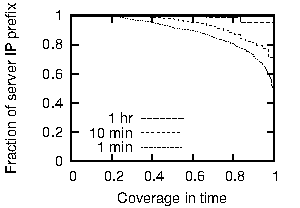
\includegraphics[width=140pt]{data2/serverPrefix-test-city.pdf}
}
\hspace{-0.5cm}
\subfigure[Pair of /24 prefix btw. client and server]
{
	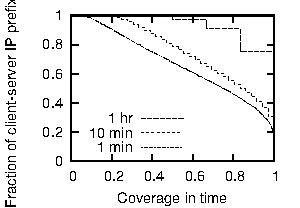
\includegraphics[width=140pt]{data2/cdf-test-asnServerPrefix.pdf}
}
\vspace{-0.1cm}
\tightcaption{Inverse CDF of server-side coverage (fraction of server-side IP prefix and server-client pairs which can be consistently measured) -- Above 55\% of observed server IP prefix and 20\% of server-client pairs can be measured in every minute. }
\label{fig:video:server-coverage}
\end{figure}

\begin{figure}[t!]
\centering
\subfigure[IP links]
{
	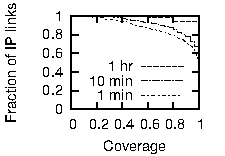
\includegraphics[width=120pt]{data2/cdf-test-link.pdf}
}
\hspace{-0.7cm}
%\subfigure[AS links (inter-domain links)]
%{
%	
\includegraphics[width=220pt]{figures/empty-figure.pdf}
%}
%\hspace{-0.5cm}
\subfigure[\# of concurrent sessions on each link]
{
	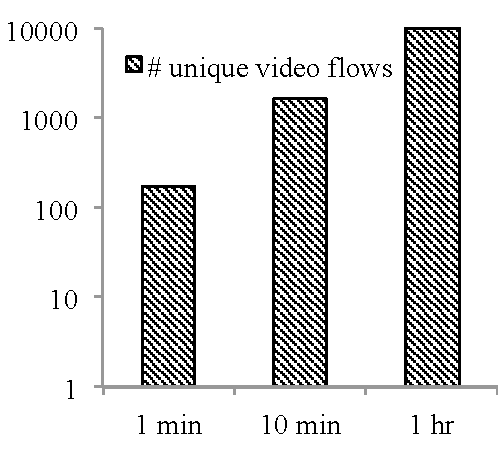
\includegraphics[width=110pt]{figures/link-load.pdf}
\label{fig:video:path-coverage-2}
}
\vspace{-0.3cm}
\tightcaption{Inverse CDF of fraction of IP links that can be consistently measured -- More than 60\% of observed links can be measured in every minute, with a median traffic volume of 170 unique video sessions in a one-minute time window.}
\label{fig:video:path-coverage}
\end{figure}

\subsection{Link coverage} Now we would like to investigate the coverage inside the network. Figure~\ref{fig:video:path-coverage} presents the inverse CDF of link coverage using the same methodology as in Figure~\ref{fig:video:client-coverage}. 
It is shown that more than 60 \% of observed links can be consistently probed in every minute. 
We also examine the traffic volume (i.e., number of current video sessions) we manage to measure on each link within different time granular. Figure~\ref{fig:video:path-coverage-2} shown that the median number of different current video sessions on each link during a time window of 1 minute, 10 minutes or one hour. The figure shows that each link will be probed every minute by 170 video sessions in median.

\subsection{Main observations}

In summary, we observe that by passively measuring the video traffic, 40 \% of
client-side AS can be measured with at least 50 simultaneous sessions in every
10 minutes and 36 \% of these can be even measured in every minutes. Moreover,
more than 30 \% of the paths from client IP prefix to server IP prefix in the
dataset is probed every 10 minutes with at least 50 simultaneous sessions.  




\section{System Overview}
\label{sec:overview}
% of a Real-time Traffic Map}


\begin{figure}[t!]
\centering
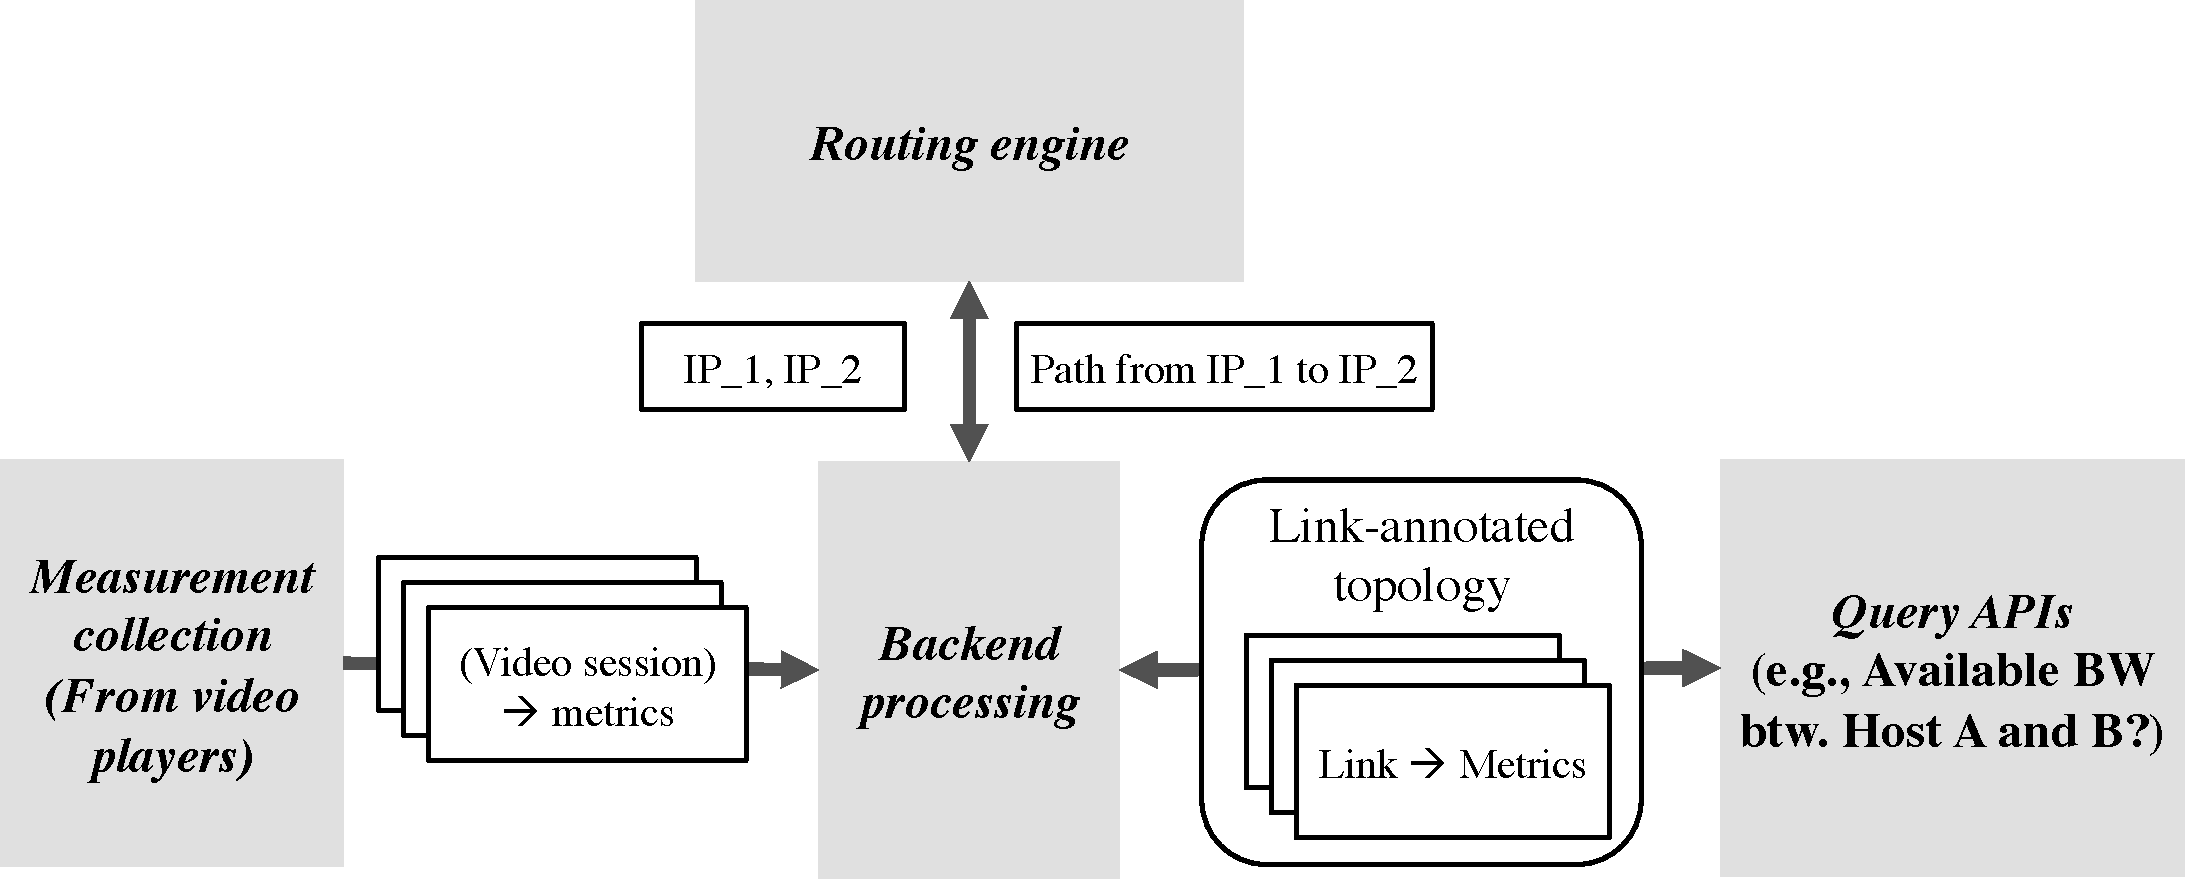
\includegraphics[width=230pt]{figures/system_overview_short.pdf}
\vspace{-0.3cm}
\tightcaption{High level components a Real-time Traffic Map. The {\it measurement engine} gathers raw data of application-layer metrics (e.g., download speed) from client-side video players, and then the {\it backend processing} combines the performance between server and client with their paths obtained by looking up the {\it routing engine} to generate a link-annotated graph. The link-annotated graph can be used to predict answer {\it query APIs} such as bandwidth between two given hosts.}
\label{fig:overview:system}
\end{figure}

Our overarching vision is to create a {\em  Real-time Traffic Map (RTM)}
 as shown in Figure~\ref{fig:overview:system}. The RTM is a
service that applications can query using a public API to obtain a near
real-time available bandwidth estimate between arbitrary pairs of end hosts.
 The key enabler  is to use the massive video-based measurements collected 
  to obtain a simultaneous and collective view over the Internet with
a great coverage offered by the video traffic.  These  measurements 
 are used in conjunction with other routing engines such as 
 iPlane to ultimately a generate an annotated topology map for the 
 Internet.

 
As discussed earlier, such a service can benefit many distributed applications.
For example, CDN re-direct client requests to edge servers based on the
performance predicted between the client and servers with the replica of
requests. Likewise, many of today's video players~\cite{hds,netflix} request
content dynamically from multiple CDNs.  Peer-to-peer file distribution and
overlay multicast can benefit from peer-selection based on real-time
information of available bandwidth between two hosts. 

%What RTM provides is the technique base for building up such service. In reality, 


We envision different operational models  for such a service in practice.   Our
vision is broad enough and the RTM can be operated by different entities who
have access to video player performance.  These include video content
providers, CDN, or third-party companies. And it has been shown feasible as
some companies (e.g., Akamai) have been collecting performance characteristics
from video players for different purposes. The coverage of the RTM service
operated by different parties may depend on their visibility -- for example,
CDNs have the view of all traffic from its own servers, while content provider
may leverage the opportunities of using multiple CDNs to obtain a different
visibility. As such our focus in this paper is on establishing the technical
basis for such an RTM rather than the economics or service-level aspects.

Unlike existing systems such iPlane which leverages on a few fully controlled
nodes to carry out fine-grain (packet-level) probing and measurement, we measure
the video traffic from the view of massive video players to collect bandwidth
information. However, this poses new challenges in two aspects.

\mypara{Coarse measurement} While our approach achieves better coverage, the
measured bandwidth between two hosts will be in much more coarse-grain, because
the video players run within the browser sandbox in  application-layer and have
little knowledge of packet-level statistics. This means the bandwidth will be
measured over a coarser time duration than that of packet dispersion techniques like
Spruce~\cite{strauss2003measurement}, IGI~\cite{hu2003evaluation}.  Moreover, caching effect also
impacts the measured bandwidth, since CDNs often fetch video content from
different servers or even from a local copy.

\mypara{End-to-end measurement} Because of the sandbox limitation, it is
infeasible to collect path information by traceroute video players. So it is
challenging to predict the bandwidth between two hosts that have never been
probed by video traffic. For example, we can have bandwidth information between
each of two clients and a server, but it is very likely that the two clients
have never been probed from one to another.


\mypara{Near real-time response} Instead of managing updates from a few
machines, our approach has to handle concurrent client-side measurement from
millions of video viewers, maintain the most up-to-date information of paths
and links, and process a large number of queries in nearly real-time. We
postpone the discussion of scalability issues to Section~\ref{sec:disc}.


Ideally, like iPlane, to predict available bandwidth between hosts that have never been probed, RTM can adopt the idea of structural prediction in which
a link-annotated map is first generated and the prediction of path performance
is made by composing the segments (e.g., links) pre-calculated on the map. To
this end, we have to first identify the path which each end-to-end measurement
is using. Several existing systems provide such service; e.g., 
iPlane predicts current IP level route between any two hosts by
concatenating paths observed in traceroute data. 

With the path information, the measured metrics
associated to paths need to be converted to metrics associated to more basic
composable unit (i.e., link) which can be later composed to predict metrics of
a path that may have never been probed before.

This is challenging since we receive only application-level bandwidth
measurement. However, we can compensate the coarse-grain input with the massive
simultaneous vantage view of video traffic. The high-level idea is to combine
the routing information and bandwidth measurement using some extrapolation logic
that exploits the correlation of the massive simultaneous probes from different
paths to obtain link-level information. We present the technique in the next section.

\section{Feasibility of extrapolating links by paths}
\label{sec:ideas}

Our ultimate goal is to predict available bandwidth between two hosts by combining the 
end-to-end measurements from multiple video viewers and the
 routing information supplied by the routing engine. 


At first glance, it may appear that we need to  first extrapolate the available
bandwidth on {\em every link} in the network to predict the performance between
an arbitrary pair of  hosts.  However, in reality, it is sufficient to know
which link on the path between the two hosts is the {\em bottleneck} link and
focus only on estimating the available bandwidth of the bottleneck link.
Therefore, instead of an ``atlas'' where every link is annotated with its
available bandwidth, it suffices to have a  ``congestion map'' where only
bottleneck links are annotated with available bandwidth (generating congestion map using packet-level techniques has been studied in~\cite{dinu2011inferring}).  


 Having thus reformulated our problem, there are three conceptual steps in converting the end-to-end measurements to
the available bandwidth on the observed set of bottleneck links (i.e., to be determined) to create this
 intermediary step of a ``real-time congestion map''. Given 
 this congestion map, we can simply predict the minimum 
across all observed bottlenecks on a given end-to-end path   as the available bandwidth for that path.
 (Note that  a link may be a bottleneck for some path but it need not be the minimal bottleneck 
 for a different path.)


\begin{packeditemize}

	\item First, the  measurement from each video session is associated with the server and client IP (or AS depending on how much information the underlying streaming protocols provide). 

	\item Second, the client-server IP pairs are then mapped to link-level paths via routing information provided by other services (e.g., iPlane).

	\item Finally, we use an extrapolation algorithm to infer available bandwidth of all bottleneck links to generate a congestion map. In addition, the congestion map also include the information that all links along the path have at least the available bandwidth of the bottleneck link.

\end{packeditemize}


\begin{figure}[h!]
\begin{center}
%\includegraphics[]{p1_2Fig.ps}
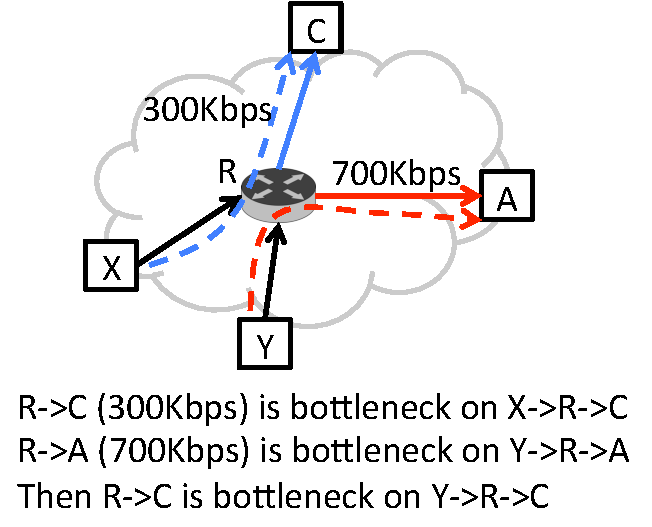
\includegraphics[scale=0.5] {figures/congestion_map.pdf}
\vspace{-0.4cm}
\caption{Example of congestion map. The available bandwidth between Y and C is calculated based on the congestion map -- Link YC has larger bandwidth than RA which is above RC, therefore, RC is bottleneck and available bandwidth of path Y to C is 300Kbps.}
\label{fig:idea:example}
\end{center}
\end{figure}

The key technique to identify bottleneck links for paths, called ``bottleneck
inference'', exploits the power of large number of overlapping paths,
and annotated the available bandwidth of the bottleneck link with the available
bandwidth of the path.  When given the path between two IP addresses, we
compare the available bandwidth of every link along it to identify the bottleneck link
with the lowest available bandwidth, and output that as the predicted available
bandwidth between the two IP addresses. Figure~\ref{fig:idea:example} shows how congestion map is used to identify bottleneck link and available bandwidth between two hosts.

%We now focus on the bottleneck
%inference technique. 
%We will use real topology and different traffic patterns to
%test its accuracy in identifying the bottlenecks and its coverage in predicting the
%available bandwidth for any two hosts as well. 
%\vyas{this only obtains bandwidth for the bottlenck links -- what about
%others}


\subsection{Bottleneck inference}
The basic idea of bottleneck inference algorithm is to rank the IP-level links
along the routing path of each session by the likelihood for it to be the bottleneck
link, and the likelihood is called {\it Bottleneck Score} (similar to ~\cite{agarwal2010webprofiler}). Note that only using this technique, we
cannot pinpoint which link is the bottleneck. Instead, this technique
enables to identify the link that is most likely to be the bottleneck
(i.e., with highest Bottleneck Score). 

The algorithm is based on two assumptions:
\begin{packeditemize}
	\item {\bf A1:} The available bandwidth of a path is identical to that of the bottleneck link, and 
	\item {\bf A2:} (Fair sharing) All paths sharing the same bottleneck link should receive at most the available bandwidth on the link.
\end{packeditemize}
Consequently, we have the following statements: ``{\it Given two paths $P,P'$ such that $P$ shares a link $L$ with $P'$, if $P'$ has a significantly higher bandwidth than $P$, then the bottleneck link of $P$ should not be $L$}''. The rationale is that if otherwise, $P$ is bottlenecked by link $L$, $P'$ should get at most the available bandwidth of $L$ ({\bf A2}) which is identical to the bandwidth seen by $P$ ({\bf A1}). However, this is contradict to the assumption. 
More realistically, taking into account other  parameters (e.g., round trip time, slow start time), the bandwidth $P'$ sees could be a bit different from what $P$ sees. So we only consider cases where $P'$ has bandwidth significantly higher (e.g., 50\% higher) than $P$. For example, in Figure~\ref{fig:idea:example}, since path from  $B$ to $D$ (10Mbps) has significantly higher bandwidth than from $A$ to $C$ (100Kbps), their overlapping link between $E$ and $F$ should not be the bottleneck of path from $A$ to $C$.

\begin{figure}[h]
\begin{center}
%\includegraphics[]{p1_2Fig.ps}
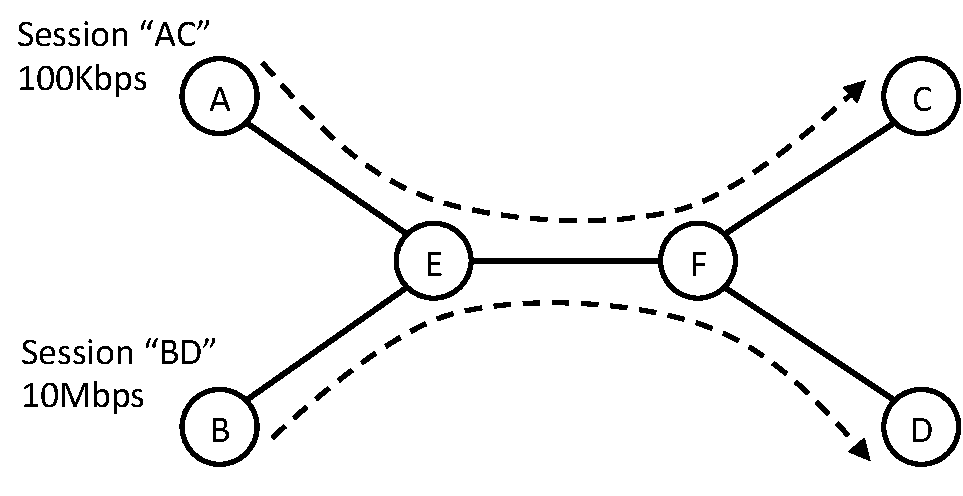
\includegraphics[scale=0.4] {figures/bottleneckExample.pdf}
\vspace{-0.5cm}
\caption{Simple example of bottleneck inference algorithm.}
\label{fig:idea:example}
\end{center}
\end{figure}

Based on this intuition, we calculate a Bottleneck Score for each link along a path that indicates how likely the link is to be a bottleneck as follows. Suppose that each path $P$ is a set of links along it, and for each link $L$ on path $P$, its Bottleneck Score is:
\begin{align*}
&BottleneckScore(L)\\
&=1-Pr\{BW(P') > 150\%\cdot BW(P) | L \in P \cap P'\}\\
&=1-\frac{|\{P'|\{BW(P') > 150\%\cdot BW(P), L \in P \cap P'\}|}{|\{P'|L \in P \cap P'\}|}
\end{align*}

Intuitively, the higher the Bottleneck Score is, the less the fraction of other paths indicating the link not being a bottleneck is, and thus in other words, the more likely the link is the bottleneck. The technique will return the links with the highest score. 
One thing needs to note is that if a link is not shared with other path (i.e., $\{P'|L\in P\cap P'\}=\emptyset$), the Bottleneck Score will become meaningless. This is usually caused by last mile links that only connect to a few users.
To avoid this problem, we aggregage client and server IP into /24 blocks, and predict the bottleneck along the path between two IP blocks. 


%We note that bottleneck link identification via path correlation has been studied before (e.g., \cite{agarwal2010webprofiler})


%% VS: either flesh this related work or dont say anything
%To rule out p
%ossible bottleneck link by correlating paths is not first proposed -- \cite{} has mentioned the same idea and \cite{} used path comparison to find system bottleneck in other scenarios. However, our contribution lies in ...

\begin{figure}[h]
\begin{center}
%\includegraphics[]{p1_2Fig.ps}
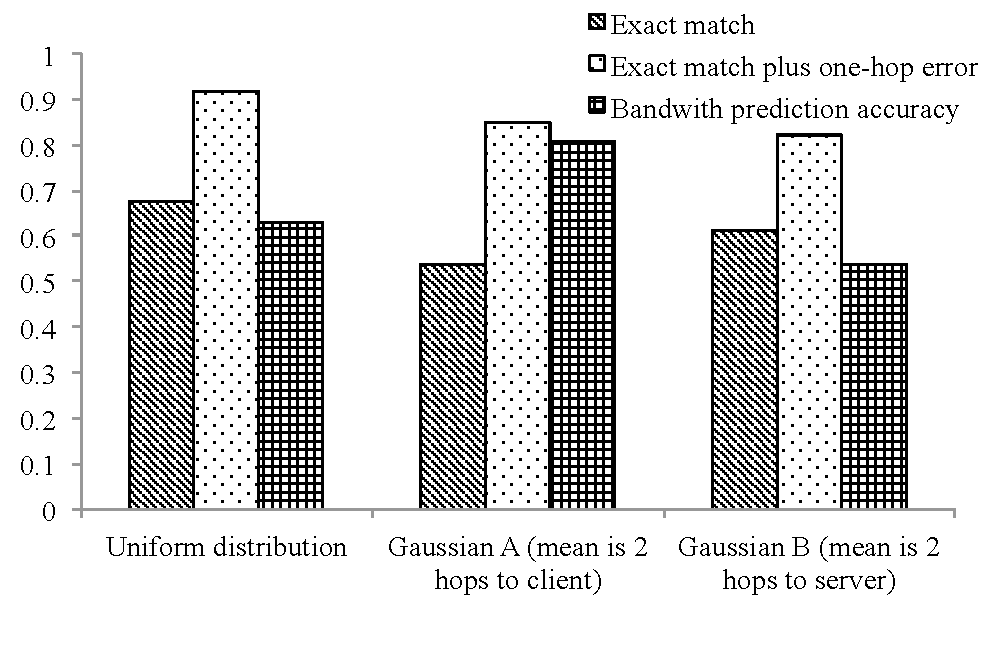
\includegraphics[scale=0.4] {figures/bottle-sim-bar-w-prediction.pdf}
\vspace{-0.9cm}
\caption{Simulation-based validation for bottleneck inference technique.}
\label{fig:cdn-criticalAttributeSets}
\end{center}
\end{figure}

\subsection{Simulation-based validation}
We now use a data-driven simulation to validate the proposed bottleneck
inference technique. The goal of the simulation is
to test the feasibility of bottleneck inference -- (i) how accurate it is to identify
bottleneck links in a real topology and various bottleneck distribution, and (ii) how accurate it is to use the identified bottlenecks to predict available bandwidth of any two hosts.

To this end, we use client requests in our own dataset and the path obtained
from iPlane to generate a real network topology of links that have been probed
by video sessions. We then randomly generate sessions between client and
servers by three bottleneck distributions -- uniformly
distribution through the network, skewed distribution such that bottlenecks are
closer to clients, and that bottlenecks are closer to
servers. To control the location of bottleneck for each session, we adjust the
volume of background traffic on each link. Finally, we run the bottleneck inference algorithm 
to localize the bottleneck links based on bandwidth seen by edge users and compare it with the ground truth.
Figure~\ref{fig:cdn-criticalAttributeSets} present the result under three bottleneck distributions. Each of them has run for
30 times and we show the average value. 

The first two bars show the bottleneck identification accuracy -- it is consistent that more than 80\% of the identified bottlenecks
are no more than 1 hop from the real bottlenecks. This error is tolerable in the hope
that one hop will not significantly change the location of the bottleneck
links. 
The last bar shows the bandwidth estimation accuracy -- we use the obtained congestion map to predict the available bandwidth between all pairs of edge users and compare it with the ground truth. It shows the accuracy (with less than 10\% error) also achieves as high as 80\%.


In summary, we find that by correlating views from multiple concurrent video flows, we are able to quite accurately locate bottleneck links, and based on these revealed bottleneck links (i.e., congestion map), the available bandwidth between any two hosts can be predicted with descent accuracy even with a simple unoptimized heuristic approach. We believe that we can further improve this with better estimation/laerning techniqies.

\section{Discussion}
\label{sec:disc}

\mypara{Coverage gaps} Even though we saw in Section 2 that a video analytics
 provider has sufficient coverage, we may still have ``gaps'' in our traffic map; e.g.,
 some links may be missing or our data might be stale. One approach to fill in these 
gaps is to use models of historic behavior (e.g., stability of the link's available 
 bandwidth or time-of-day effects) to  improve the accuracy of predictions.

\mypara{Improving the routing engine} Systems such as iPlane have already taken
a significant first step toward providing a good understanding of the routing
behavior of the Internet. That said, in our early experiments we found that
there are substantial ``holes'' in the topology maps, especially in the context
of the client-server patterns we observe with video viewers requesting content
from CDNs. Thus, a natural next step will be to provide mechanisms to improve
the accuracy and coverage of the path prediction mechanisms as well. Here, we see a natural
synergy---the video measurements can in fact serve as a feeder to improve the
routing engine. For instance, this data can help bootstrap the routing engine
with more IP pairs and also  ``triggering'' new measurements whenever there are
significant ``holes'' in the topology maps. 
 

\mypara{A federated model} So far, we considered a centralized operation model
where a single service provider collects and ``owns'' the video data to offer
the RTM service. It is possible that we can dramatically improve the coverage
if a small number of large providers cooperatively share the individual RTMs in
a loosely federated manner. One concern, however, is whether this type of
sharing may reveal proprietary information; e.g., CDN server selection
strategies and thus we would need corresponding mechanisms to prevent such
accidental information leakage. 

\mypara{Scalability}  Our goal so far has largely been to establish the viability 
 of implementing a RTM service and we have not focused on the scalability, either 
of the data collection or of the bottleneck inference steps. A natural question 
 is if there are simple optimizations (e.g., sending ``diff''s or only 
 reporting significant deviations from previous reports) in the measurement 
 engine. Similarly, another question is whether the mapping and extrapolation 
 logic can be distributed (e.g., using MapReduce or other parallelization 
solutions).

%\subsection{Backend scalability}

%\subsection{Biased visibility of Internet}

%\subsection{More accurate routing engine}

%\subsection{Privacy issues}

%\subsection{Distributing lightweight measurement code}

\section{Conclusion}
\label{sec:concl}

 Our vision here is a real-time traffic map for the Internet that different
applications query for different path properties and use them to inform their
decisions (e.g., server or peer selection). The key enabler here is the growth
of Internet video and the deployment of measurement instrumentation as part of
the video player logic that can address key issues w.r.t\ coverage, real-time
updates, and the ability to measure bandwidth with close-to-zero overhead. That
said, the inability to collect fine-grained and adaptive measurements introduce
challenges in translating the potential of using video-based measurements.
Fortunately, we show that we can compensate for this lack of  instrumentation
by correlating coarse views collected from multiple diverse vantage points to
identify bottleneck links in the network. 


{\scriptsize
\bibliographystyle{abbrv}
\bibliography{adaptation,sigcomm2011,sigcomm2012,sigcomm2013,conext13,hotnet13.bib}
}

\end{document}

